\documentclass[a4paper]{article}

\usepackage{geometry}

\usepackage{caption}
\usepackage{amsmath}

\captionsetup[table]{position=bottom}

%\usepackage[cm]{fullpage}

% some very useful LaTeX packages include:

%\usepackage{cite}      % Written by Donald Arseneau
                        % V1.6 and later of IEEEtran pre-defines the format
                        % of the cite.sty package \cite{} output to follow
                        % that of IEEE. Loading the cite package will
                        % result in citation numbers being automatically
                        % sorted and properly "ranged". i.e.,
                        % [1], [9], [2], [7], [5], [6]
                        % (without using cite.sty)
                        % will become:
                        % [1], [2], [5]--[7], [9] (using cite.sty)
                        % cite.sty's \cite will automatically add leading
                        % space, if needed. Use cite.sty's noadjust option
                        % (cite.sty V3.8 and later) if you want to turn this
                        % off. cite.sty is already installed on most LaTeX
                        % systems. The latest version can be obtained at:
                        % http://www.ctan.org/tex-archive/macros/latex/contrib/supported/cite/
\usepackage[inline]{enumitem}

\usepackage{graphicx}   % Written by David Carlisle and Sebastian Rahtz
                        % Required if you want graphics, photos, etc.
                        % graphicx.sty is already installed on most LaTeX
                        % systems. The latest version and documentation can
                        % be obtained at:
                        % http://www.ctan.org/tex-archive/macros/latex/required/graphics/
                        % Another good source of documentation is "Using
                        % Imported Graphics in LaTeX2e" by Keith Reckdahl
                        % which can be found as esplatex.ps and epslatex.pdf
                        % at: http://www.ctan.org/tex-archive/info/

%\usepackage{psfrag}    % Written by Craig Barratt, Michael C. Grant,
                        % and David Carlisle
                        % This package allows you to substitute LaTeX
                        % commands for text in imported EPS graphic files.
                        % In this way, LaTeX symbols can be placed into
                        % graphics that have been generated by other
                        % applications. You must use latex->dvips->ps2pdf
                        % workflow (not direct pdf output from pdflatex) if
                        % you wish to use this capability because it works
                        % via some PostScript tricks. Alternatively, the
                        % graphics could be processed as separate files via
                        % psfrag and dvips, then converted to PDF for
                        % inclusion in the main file which uses pdflatex.
                        % Docs are in "The PSfrag System" by Michael C. Grant
                        % and David Carlisle. There is also some information
                        % about using psfrag in "Using Imported Graphics in
                        % LaTeX2e" by Keith Reckdahl which documents the
                        % graphicx package (see above). The psfrag package
                        % and documentation can be obtained at:
                        % http://www.ctan.org/tex-archive/macros/latex/contrib/supported/psfrag/

%\usepackage{subfigure} % Written by Steven Douglas Cochran
                        % This package makes it easy to put subfigures
                        % in your figures. i.e., "figure 1a and 1b"
                        % Docs are in "Using Imported Graphics in LaTeX2e"
                        % by Keith Reckdahl which also documents the graphicx
                        % package (see above). subfigure.sty is already
                        % installed on most LaTeX systems. The latest version
                        % and documentation can be obtained at:
                        % http://www.ctan.org/tex-archive/macros/latex/contrib/supported/subfigure/

\usepackage{url}        % Written by Donald Arseneau
                        % Provides better support for handling and breaking
                        % URLs. url.sty is already installed on most LaTeX
                        % systems. The latest version can be obtained at:
                        % http://www.ctan.org/tex-archive/macros/latex/contrib/other/misc/
                        % Read the url.sty source comments for usage information.

%\usepackage{stfloats}  % Written by Sigitas Tolusis
                        % Gives LaTeX2e the ability to do double column
                        % floats at the bottom of the page as well as the top.
                        % (e.g., "\begin{figure*}[!b]" is not normally
                        % possible in LaTeX2e). This is an invasive package
                        % which rewrites many portions of the LaTeX2e output
                        % routines. It may not work with other packages that
                        % modify the LaTeX2e output routine and/or with other
                        % versions of LaTeX. The latest version and
                        % documentation can be obtained at:
                        % http://www.ctan.org/tex-archive/macros/latex/contrib/supported/sttools/
                        % Documentation is contained in the stfloats.sty
                        % comments as well as in the presfull.pdf file.
                        % Do not use the stfloats baselinefloat ability as
                        % IEEE does not allow \baselineskip to stretch.
                        % Authors submitting work to the IEEE should note
                        % that IEEE rarely uses double column equations and
                        % that authors should try to avoid such use.
                        % Do not be tempted to use the cuted.sty or
                        % midfloat.sty package (by the same author) as IEEE
                        % does not format its papers in such ways.
\usepackage{amssymb}
\usepackage{amsmath}    % From the American Mathematical Society
                        % A popular package that provides many helpful commands
                        % for dealing with mathematics. Note that the AMSmath
                        % package sets \interdisplaylinepenalty to 10000 thus
                        % preventing page breaks from occurring within multiline
                        % equations. Use:
%\interdisplaylinepenalty=2500
                        % after loading amsmath to restore such page breaks
                        % as IEEEtran.cls normally does. amsmath.sty is already
                        % installed on most LaTeX systems. The latest version
                        % and documentation can be obtained at:
                        % http://www.ctan.org/tex-archive/macros/latex/required/amslatex/math/
\usepackage{latexsym}
\usepackage{amsthm}

\usepackage{verbatim}

\usepackage[utf8]{inputenc}
\usepackage[italian]{babel}

\usepackage[htt]{hyphenat}

\hyphenation{en-ter-crit-i-cal-sec-tion}
\hyphenation{ex-it-crit-i-cal-sec-tion}

\setcounter{secnumdepth}{4}

\setlength{\parindent}{0pt}

\usepackage{algorithm}
\usepackage{algpseudocode}
\algrenewcommand{\algorithmiccomment}[1]{$\left(\text{#1}\right)$}

\usepackage{color}

\definecolor{ideanumber}{rgb}{0.0,0.0,1.0}
\definecolor{ideacomment}{rgb}{0.5,0.5,0.5}
\definecolor{ideakeyword}{rgb}{0.0,0.0,0.5}
\definecolor{ideastring}{rgb}{0.0,0.5,0.0}

\usepackage{listings}
\lstset{frame=tb,
    language=Java,
    aboveskip=3mm,
    belowskip=3mm,
    showstringspaces=false,
    columns=flexible,
    basicstyle={\small\ttfamily},
    numbers=left,
    numbersep=2pt,                   % how far the line-numbers are from the code
    numberstyle=\tiny\color{ideacomment},
    keywordstyle=\color{ideakeyword},
    commentstyle=\color{ideacomment},
    stringstyle=\color{ideastring},
    breaklines=true,
    breakatwhitespace=true,
    tabsize=4
}

% Other popular packages for formatting tables and equations include:

%\usepackage{array}
% Frank Mittelbach's and David Carlisle's array.sty which improves the
% LaTeX2e array and tabular environments to provide better appearances and
% additional user controls. array.sty is already installed on most systems.
% The latest version and documentation can be obtained at:
% http://www.ctan.org/tex-archive/macros/latex/required/tools/

% V1.6 of IEEEtran contains the IEEEeqnarray family of commands that can
% be used to generate multiline equations as well as matrices, tables, etc.

% Also of notable interest:
% Scott Pakin's eqparbox package for creating (automatically sized) equal
% width boxes. Available:
% http://www.ctan.org/tex-archive/macros/latex/contrib/supported/eqparbox/

% *** Do not adjust lengths that control margins, column widths, etc. ***
% *** Do not use packages that alter fonts (such as pslatex).         ***
% There should be no need to do such things with IEEEtran.cls V1.6 and later.
\newcommand\textsup[1]{$^{\text{#1}}$}
\newcommand\textsub[1]{$_{\text{#1}}$}

% Define document title and author
\title{\Huge \bf
Assignment \#4
}
\author{
    Martina Magnani\\
    \texttt{martina.magnani8@studio.unibo.it}
    \and
    Nicola Piscaglia\\
    \texttt{nicola.piscaglia2@studio.unibo.it}
    \and
    Mattia Vandi\\
    \texttt{mattia.vandi@studio.unibo.it}
}
\date{}

% Your document starts here!
\begin{document}

\maketitle

%\tableofcontents

\section{Analisi del problema}\label{analisi-del-problema-1}
Implementare un servizio di chat distribuito, prendendo come riferimento le architetture orientate ai servizi e reattive e aspetti metodologici correlati.

Il servizio di chat deve permettere di creare dinamicamente nuove chat, per ognuna delle quali valgono i requisiti specificati nell'Assignment 03:
\begin{itemize}
    \item Un utente può aggiungersi e rimuoversi dinamicamente.
    \item Ogni messaggio inviato da un utente deve essere visualizzato da tutti gli altri utenti.
    \item Il sistema deve essere completamente decentralizzato.
        \begin{itemize}
            \item A parte, eventualmente, la presenza di un (attore) registro con indirizzo/nome noto che tenga traccia dei partecipanti.
        \end{itemize}
    \item I messaggi inviati nella chat devono essere visualizzati da tutti i partecipanti nel medesimo ordine.
\end{itemize}
Supporto per una modalità “sezione critica”:
\begin{itemize}
    \item Un partecipante può chiedere di entrare in sezione critica inserendo un comando predefinito.
    \item Quando un partecipante entra in sezione critica, possono essere visualizzati solo i suoi messaggi, senza intervallarli a quelli degli altri utenti.
    \item Un solo partecipante alla volta può essere in sezione critica.
    \item Per uscire dalla sezione critica si può prevedere un altro comando predefinito (es: “:exit-cs”).
    \item Un utente può rimanere in sezione critica per un certo tempo massimo Tmax, dopodiché l'uscita è forzata.
    \item Durante una sezione critica i messaggi inviati dagli altri partecipanti devono essere rigettati.
\end{itemize}

Il servizio può avere un front-end di qualsiasi tipo (a linea di comando, GUI, web-based).

Il servizio deve essere progettato mettendo in campo un'architettura che consideri aspetti non funzionali quali:
\begin{itemize}
    \item scalabilità (all'aumentare del numero di chat e del numero di utenti per chat),
    \item resilienza,
    \item responsività.
\end{itemize}

\section{Descrizione della soluzione proposta}\label{soluzione-proposta}

\subsection{Architettura del sistema}\label{architettura-del-sistema}
Ad alto livello il sistema è formato da due macrocomponenti: un \textit{Web Server} ed un \textit{Web Client} (di seguito chiamato \texttt{ChatClient}). 
Il \textit{Web Server} è stato organizzato utilizzando l'architettura a microservizi. In particolare, i servizi presenti nella nostra soluzione sono:
\begin{itemize}
    \item \texttt{UserService}: gestisce le operazioni di memorizzazione/lettura dei dati degli utenti.
    \item \texttt{RoomService}: gestisce lo stato delle chat distribuite.
   \item \texttt{WebAppService}: gestisce la comunicazione del client web con gli altri servizi.
   \item \texttt{HealthCheckService}: controlla la disponibilità dei vari servizi.
\end{itemize}
 
\subsection{Dinamica del sistema}\label{dinamica-del-sistema}
Ogni servizio espone una propria interfaccia REST per poter essere contattato dagli altri servizi.

La dinamica del sistema è stata rappresentata ad alto livello con diagrammi di sequenza, adatti per mostrare in modo efficace lo scambio di messaggi tra le entità del sistema.

Ogni interazione fra servizi è preceduta da una verifica della disponibilità del servizio effettuata dall'\texttt{HealthCheckService}.

Di seguito vengono mostrati i principali scenari d'interazione.

\begin{figure}[H]
    \centering
    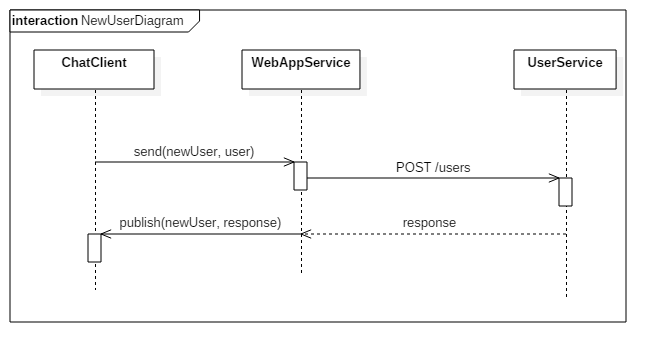
\includegraphics[width=\linewidth, height=\textheight, keepaspectratio]{res/NewUserDiagram.png}
    \caption{Diagramma di sequenza che mostra la registrazione di un nuovo utente.}
    \label{fig:new-user-diagram}
\end{figure}

Nell'interazione descritta in figura \ref{fig:new-user-diagram} l'interazione fra i vari servizi è la seguente:
\begin{enumerate*}[label=(\arabic*)]
%
    \item l'utente effettua il login sull'applicazione client (\texttt{ChatClient});
%
    \item il client pubblica l'evento sull'Event Bus;
%
    \item il servizio (\texttt{WebAppService}) in ascolto sul canale inoltra il messaggio allo \texttt{UserService};
%
    \item lo \texttt{UserService} crea il nuovo utente e risponde con il risultato dell'operazione.
\end{enumerate*}

\begin{figure}[H]
    \centering
    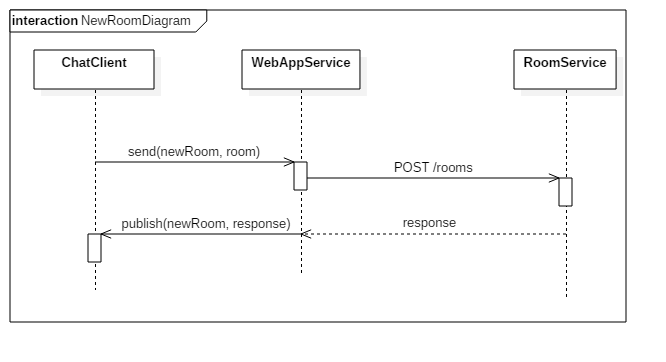
\includegraphics[width=\linewidth, height=\textheight, keepaspectratio]{res/NewRoomDiagram.png}
        \caption{Diagramma di sequenza che mostra la creazione di una stanza.}
    \label{fig:new-room-diagram}
\end{figure}

Nell'interazione descritta in figura \ref{fig:new-room-diagram} la sequenza di messaggi scambiati è la sequente:
\begin{enumerate}[label=(\arabic*)]
%
    \item il client pubblica l'evento sull'Event Bus;
%
    \item il servizio (\texttt{WebAppService}) in ascolto sul canale inoltra il messaggio al \texttt{RoomService};
    
    \item il \texttt{RoomService} crea la nuova stanza e risponde con il risultato dell'operazione.
\end{enumerate}

\begin{figure}[H]
    \centering
    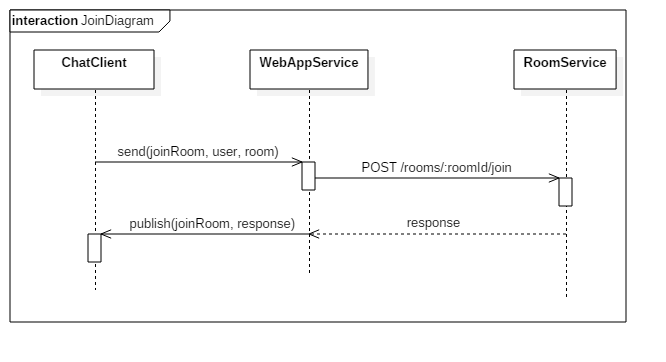
\includegraphics[width=\linewidth, height=\textheight, keepaspectratio]{res/JoinDiagram.png}
        \caption{Diagramma di sequenza che mostra l'entrata di un utente in una stanza.}
    \label{fig:enter-diagram}
\end{figure}

Nell'interazione descritta in figura \ref{fig:enter-diagram} la sequenza di messaggi scambiati è la sequente:
\begin{enumerate*}[label=(\arabic*)]
%
    \item il client pubblica l'evento sul canale, mostrando l'intenzione dell'utente di entrare/uscire dalla stanza;
%
    \item il \texttt{WebAppService} in ascolto sul canale inoltra il messaggio al \texttt{RoomService};
%   
    \item il \texttt{RoomService} aggiunge/rimuove l'utente alla/dalla stanza e risponde con il risultato dell'operazione.
%
\end{enumerate*}

\begin{figure}[H]
	\centering
	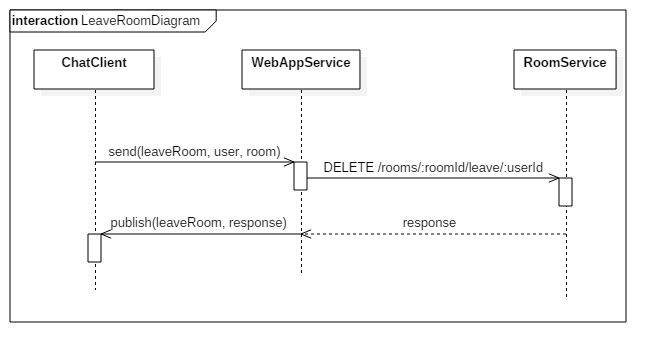
\includegraphics[width=\linewidth, height=\textheight, keepaspectratio]{res/LeaveRoomDiagram.png}
	\caption{Diagramma di sequenza che mostra l'uscita di un utente da una stanza.}
	\label{fig:leave-diagram}
\end{figure}

\begin{figure}[H]
    \centering
    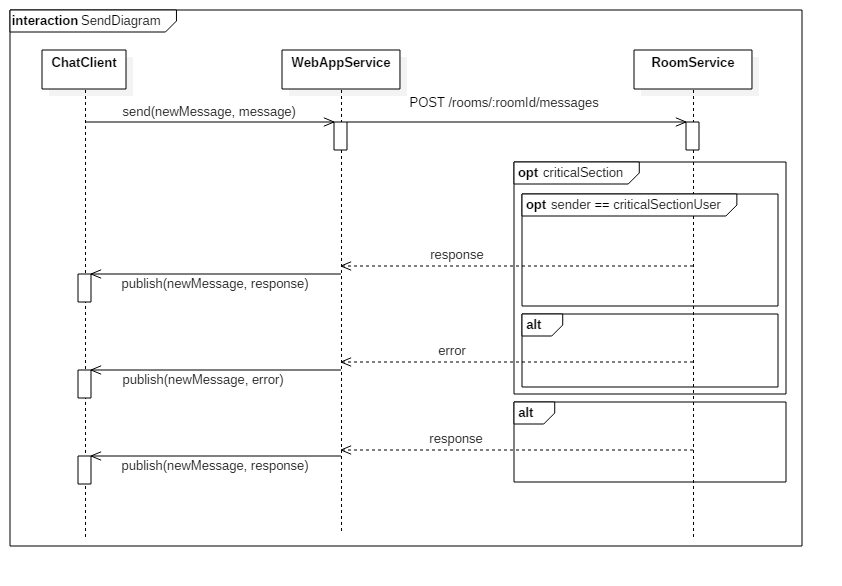
\includegraphics[width=\linewidth, height=\textheight, keepaspectratio]{res/SendDiagram.png}
        \caption{Diagramma di sequenza che mostra lo scambio di messaggi fra gli utenti di una stanza.}
    \label{fig:messages-diagram}
\end{figure}


Nell'interazione descritta in figura \ref{fig:messages-diagram} la sequenza di messaggi scambiati è la sequente:
\begin{enumerate}[label=(\arabic*)]
	%
	\item Il client pubblica l'evento sull'Event Bus, mostrando l'intenzione di un utente di pubblicare un messaggio nella chat.
	%
	\item il \texttt{WebAppService} in ascolto sul canale inoltra il messaggio al \texttt{RoomService}; 
	%
	\item Nel caso in cui non ci sia una sezione critica il messaggio viene inviato a tutti gli altri client.
	%
	\item Nel caso in cui ci sia una sezione critica:
	\begin{enumerate}
		\item se il mittente è l'utente in sezione critica il messaggio viene accettato;
		%
		\item se il mittente non è l'utente in sezione critica, il messaggio viene rifiutato e viene segnalata l'impossibilità di mandare il messaggio.
		%
	\end{enumerate}
\end{enumerate}

\begin{figure}[H]
    \centering
    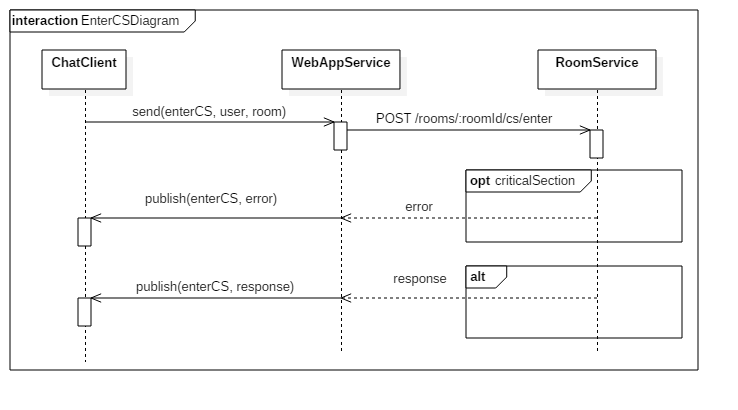
\includegraphics[width=\linewidth, height=\textheight, keepaspectratio]{res/EnterCSDiagram.png}
        \caption{Diagramma di sequenza che mostra la richiesta di entrare in sezione critica da parte di un utente.}
    \label{fig:enterCS-diagram}
\end{figure}

\begin{figure}[H]
    \centering
    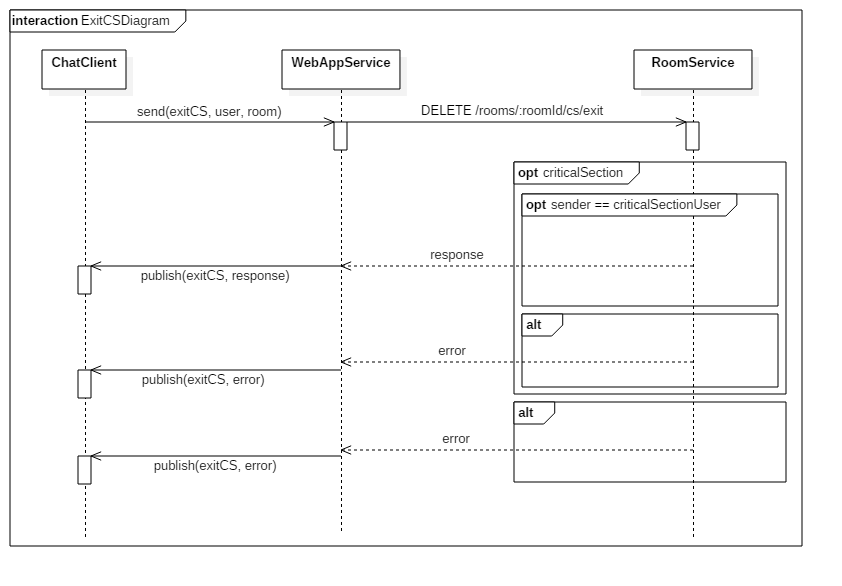
\includegraphics[width=\linewidth, height=\textheight, keepaspectratio]{res/ExitCSDiagram.png}
        \caption{Diagramma di sequenza che mostra la richiesta di uscire dalla sezione critica da parte di un utente.}
    \label{fig:exitCS-diagram}
\end{figure}


\subsection{Algoritmo di ordinamento}\label{ordinamento}

Il problema dell'ordinamento dei messaggi può essere scomposto in due sottoproblemi tra loro indipendenti:

\begin{itemize}
%
    \item\textbf{causal message ordering}: assicura che tutti i messaggi vengano elaborati secondo il loro ordine di invio;
%
    \item\textbf{total message ordering}: assicura che tutti i processi elaborino i messaggi nello stesso ordine.
%
\end{itemize}

Il problema dell'ordinamento dei messaggi è stato risolto utilizzando due algoritmi che descriviamo di seguito. Questo permette ad ogni utente di avere una visione coerente e ordinata dei messaggi.

\subsection{Causal Message Ordering}\label{causal-message-ordering}

Ogni messaggio è costituito dal testo e dal numero di sequenza associatogli dal mittente.
Ogni utente mantiene per ogni processo il numero di messaggi inviati e viene aggiornato ogni volta che l'utente è abilitato a processare il messaggio ricevuto.\\
Un utente è abilitato ad elaborare il messaggio quando il numero di sequenza all'interno del messaggio è successivo al numero di sequenza dell'ultimo messaggio elaborato per quel mittente.
Se così non fosse, significa che ci sono dei messaggi precedenti del mittente che non sono ancora stati ricevuti ed è quindi necessario attendere il loro arrivo prima di potere elaborare il messaggio appena ricevuto.
\begin{enumerate}
    \item Un processo che si unisce al sistema riceve da tutti gli altri processi il loro numero di sequenza corrente.  
    \item Un processo che invia un messaggio incrementa il proprio numero di sequenza e lo associa al messaggio. 
    \item Un processo che riceve un messaggio controlla che il numero di sequenza contenuto nel messaggio sia successivo all'ultimo numero di sequenza che ha ricevuto dal mittente.\\
    Se tale condizione è soddisfatta:
    \begin{enumerate}
        \item il messaggio viene elaborato
        \item se ci sono altri messaggi che possono essere elaborati si ritorna al punto precedente.
    \end{enumerate}
    Se tale condizione non è soddisfatta il messaggio viene aggiunto alla coda dei messaggi in attesa.
    \item Un processo che esce dal sistema viene rimosso dalle liste di tutti gli altri processi.
\end{enumerate}

\subsection{Total Message Ordering}\label{total-message-ordering}

I processi inviano i messaggi al \textit{Sequencer}: entità che assegna un numero di sequenza globale ad ogni messaggio.
%Ogni processo memorizza il numero di sequenza globale dell'ultimo messaggio elaborato.
Ogni processo mantiene un contatore che rappresenta il numero di sequenza globale dell'ultimo messaggio elaborato.

Quando un utente invia un messaggio:
\begin{enumerate}
    \item Il \textit{Sequencer} assegna al messaggio un numero di sequenza. 
    \item Un processo che riceve un messaggio controlla che il numero di sequenza del messaggio sia successivo all'ultimo numero di sequenza salvato.\\
    Se tale condizione è soddisfatta:
    \begin{enumerate}
        \item il messaggio viene elaborato
        \item se ci sono altri messaggi che possono essere elaborati si ritorna al punto precedente.
    \end{enumerate}
    Se tale condizione non è soddisfatta il messaggio viene aggiunto alla coda dei messaggi in attesa.
\end{enumerate}


\subsection{Implementazione}\label{implementazione}

La soluzione è stata implementata in linguaggio Java utilizzando la libreria Vert.x. \`E stato scelto di utilizzare Vert.x perché permette di implementare i microservizi e i pattern per la resilienza e la scalabilità in modo agile e conciso. Inoltre, rispetto a Spring e ad altri web-framework, Vert.x è una libreria leggera, asincrona e performante.\\
I servizi presenti nel sistema sono gli utenti della chat (gestiti dallo \texttt{UserService}), il gestore delle varie chat (rappresentato dal \texttt{RoomService}) e il servizio che si occupa dell'interazione con il client (rappresentato dal \texttt{WebAppService}).
 
\subsubsection{Interfacce di comunicazione}\label{interfacce-di-comunicazione}

Ogni servizio espone un'interfaccia REST HTTP che lo rende contattabile dall'esterno. Certe chiamate richiedono la trasmissione di oggetti JSON e in alcuni casi prevedono dei parametri nell'URI (preceduti dai due punti ':').  
Di seguito mostriamo i metodi esposti da ogni servizio.

\paragraph{UserService}
\begin{itemize}
    \item \texttt{POST /users}: metodo che permette la creazione di un nuovo utente.
    \begin{itemize}
        \item Richiede in ingresso un JSON contenente il nome dell'utente da creare.
        \begin{verbatim}
{
    "name": "userName"
}
        \end{verbatim}
        \item Restituisce un JSON contenente il nome e l'identificativo del nuovo utente creato.
        \begin{verbatim}
{
    "name": "userName",
    "id": 1
}
        \end{verbatim}
    \end{itemize} 
    \item \texttt{GET /users}: metodo che restituisce tutti gli utenti presenti nel sistema.
    \begin{itemize}
        \item Restituisce un array di JSON contenente gli utenti.
        \begin{verbatim}
[
    {
        "name": "userName",
        "id": 1
    },
    
    {
        "name": "userName",
        "id": 2
    },
    
    ...
]
        \end{verbatim}
    \end{itemize}
    \item \texttt{GET /users/:id}: metodo che restituisce un utente dato il suo identitificativo (id).
    \begin{itemize}
        \item Restituisce il JSON contenente l'utente richiesto.
        \begin{verbatim}
{
    "name": "userName",
    "id": 1
}
        \end{verbatim}
    \end{itemize}
    \item \texttt{PUT /users/:id}: metodo che modifica le informazioni di un utente dato il suo identitificativo (id)
    \begin{itemize}
        \item Richiede in ingresso un JSON contente il nuovo nome dell'utente da modificare.
        \begin{verbatim}
{
    "name": "newUserName"
}
        \end{verbatim}
        \item Restituisce un JSON contenente l'utente modificato.
        \begin{verbatim}
{
    "name": "newUserName",
    "id": 1
}
        \end{verbatim}
    \end{itemize}
    \item \texttt{DELETE /users/:id}: metodo che elimina un utente dato il suo identificativo (id).
    \begin{itemize}
        \item Restituisce un JSON contenente l'identificativo dell'utente eliminato.
        \begin{verbatim}
{
    "id": 1
}
        \end{verbatim}
    \end{itemize}
\end{itemize}

\paragraph{RoomService}
\begin{itemize}
    \item \texttt{POST /rooms}: metodo che permette la creazione di una nuova stanza.
    \begin{itemize}
        \item Richiede in ingresso un JSON contenente il nome della stanza da creare.
        \begin{verbatim}
{
    "name": "roomName"
}
        \end{verbatim}
        \item Restituisce un JSON contenente il nome e l'identificativo della nuova stanza creata.
        \begin{verbatim}
{
    "name": "roomName",
    "id": 1
}
        \end{verbatim}
    \end{itemize}
    \item \texttt{GET /rooms}: metodo che restituisce tutte le stanze presenti nel sistema.
    \begin{itemize}
        \item Restituisce un JSONArray contenente le stanze.
        \begin{verbatim}
[
    {
        "name": "roomName",
        "id": 1
    },
    
    {
        "name": "roomName",
        "id": 2
    },
    
    ...
]
        \end{verbatim}
    \end{itemize}
    \item \texttt{GET /rooms/:id}: metodo che restituisce una stanza dato il suo identitificativo (id).
    \begin{itemize}
        \item Restituisce il JSON contenente la stanza richiesta.
        \begin{verbatim}
{
    "name": "roomName",
    "id": 1
}
        \end{verbatim}
    \end{itemize}
    \item \texttt{PUT /rooms/:id}: metodo che modifica le informazioni di una stanza dato il suo identitificativo (id).
    \begin{itemize}
        \item Richiede in ingresso un JSON contente il nuovo nome della stanza da modificare.
        \begin{verbatim}
{
    "name": "newRoomName"
}
        \end{verbatim}
        \item Restituisce un JSON contenente la stanza modificata.
        \begin{verbatim}
{
    "name": "newRoomName",
    "id": 1
}
        \end{verbatim}
        \end{itemize}
    \item \texttt{DELETE /rooms/:id}: metodo che elimina una stanza dato il suo identificativo (id).
    \begin{itemize}
        \item Restituisce un JSON contenente l'identificativo della stanza eliminata.
        \begin{verbatim}
{
    "id": 1
}
        \end{verbatim}
    \end{itemize}
    \item \texttt{POST /rooms/:roomId/messages}: metodo che permette di aggiungere un messaggio alla chat corrispondente alla stanza con identificativo \texttt{roomId}.
    \begin{itemize}
        \item Richiede in ingresso un JSON contente l'utente che vuole inviare il messaggio, il suo clock e il contenuto del messaggio. 
        \newpage
        \begin{verbatim}
{
    "user": {
        "id": 1,
        "name": "userName"
    },
    "userClock": 3,
    "content": "This is the message content"
}
        \end{verbatim}
        \item Restituisce un oggetto JSON uguale a quello ricevuto con in aggiunta il globalCounter.
        \begin{verbatim}
{
    "user": {
        "id": 1,
        "name": "userName"
    },
    "userClock": 3,
    "content": "This is the message content",
    "globalCounter": 5
}
        \end{verbatim}
    \end{itemize}
    
    \item \texttt{POST /rooms/:roomId/join}: metodo che permette ad un utente di unirsi ad una stanza.
    \begin{itemize}
        \item Richiede in ingresso un JSON contente l'utente che vuole unirsi alla stanza.
        \begin{verbatim}
{
    "id": 1,
    "name": "userName"
}
        \end{verbatim}
        \item Restituisce un oggetto JSON contentente il global counter della stanza e la lista di tutti i clock degli utenti all'interno della stanza.
        \begin{verbatim}
{
    "globalCounter": 3,
    "usersClock": [
        {
            "user": user1,
            "userClock": 1
        }, 
        
        {
            "user": user2,
            "userClock": 2
        },
        
        ...
    ]
}
        \end{verbatim}
    \end{itemize}
    \item \texttt{DELETE /rooms/:roomId/leave/:userId}: metodo che permette ad un utente di abbandonare la stanza a cui si è già unito.
       \begin{itemize}
    	\item Restituisce un oggetto JSON vuoto in caso di successo o un JSON contenente un messaggio di errore in caso di fallimento.
	    \end{itemize}
    \item \texttt{GET /rooms/:roomId/cs}: metodo che indica se la stanza è in sezione critica o meno e, in tal caso, qual'è l'utente in sezione critica.
    \begin{itemize}
        \item Restituisce un oggetto JSON che indica se la sezione critica è stata acquisita o meno e, in tal caso, da quale utente.
        \begin{verbatim}
{
    "held": true,
    "user": {
        "id": 1,
        "name": "userName"
    }
}
        \end{verbatim}
        \item Restituisce un oggetto JSON vuoto in caso di successo o un JSON contenente un messaggio di errore in caso di fallimento.
    \end{itemize}
    \item \texttt{POST /rooms/:roomId/cs/enter}: metodo che permette ad un utente cha ha già acquisito la sezione critica in una stanza di rilasciarla.
    \begin{itemize}
        \item Richiede in ingresso un JSON contente l'utente che vuole entrare in sezione critica.
        \begin{verbatim}
{
    "id": 1,
    "name": "userName"
}
        \end{verbatim}
        \item Restituisce un oggetto JSON vuoto in caso di successo o un JSON contenente un messaggio di errore in caso di fallimento.
    \end{itemize}
    \item \texttt{DELETE /rooms/:roomId/cs/exit/:userId}: metodo che permette l'uscita dalla sezione critica.
    \begin{itemize}
        \item Restituisce un oggetto JSON vuoto in caso di successo o un JSON contenente un messaggio di errore in caso di fallimento.
    \end{itemize}
\end{itemize}

\paragraph{WebAppService}
\begin{itemize}
    \item \texttt{POST /messages}: metodo che permette di notificare il \texttt{WebAppService} qualora il timeout della sezione critica sia scaduto.
    \begin{itemize}
        \item Richiede un oggetto JSON contenente la stanza in cui è scaduta la sezione critica.
        \begin{verbatim}
{
    "id": 1,
    "name": "userName"
}
        \end{verbatim}
    \end{itemize}
\end{itemize}

\subsubsection{WebAppService e ChatClient}
Il \texttt{WebAppService} è il servizio che permette la comunicazione con il client (\texttt{ChatClient}).
La comunicazione avviene attraverso l'Event Bus di Vert.x.
Abbiamo definito un unico canale di comunicazione dal client verso il servizio e più canali di comunicazione dal servizio verso il client (uno per ogni risposta). 

Ogni messaggio che il client pubblica sull'Event Bus è definito da un JSON contenente il \textit{tipo} del messaggio e la \textit{richiesta}.
Di seguito descriviamo tutti i tipi di messaggi inviati dal client e le relative risposte. Vengono inoltre mostrati esempi delle richieste e risposte contenute nei messaggi.

\begin{itemize}

    \item \texttt{newUser}: messaggio pubblicato al momento del login di un nuovo utente.
        \begin{itemize}
            \item Contenuto del messaggio di invio:
            \begin{verbatim}
{
    "type": "newUser",
    "request": {
        name: "userName"
    } 
}
            \end{verbatim}

            \item Contenuto del messaggio di risposta:
            \begin{verbatim}
{
    "id": 1,
    "name": "userName"
}
	        \end{verbatim}         
        \end{itemize}

    \item \texttt{deleteUser}: messaggio pubblicato al momento del logout di un utente.
        \begin{itemize}
            \item Contenuto del messaggio di invio:
            \begin{verbatim}
{
    "type": "deleteUser",
    "request": {
        "userId": 1 
    } 
}
            \end{verbatim}
            \item Contenuto del messaggio di risposta:
            \begin{verbatim}
{
    "userId": 1
}
            \end{verbatim}
        \end{itemize}

    \item \texttt{rooms} : messaggio pubblicato quando un utente effettua il login in modo da ottenere le eventuali stanze presenti:
        \begin{itemize}
            \item Contenuto del messaggio di invio:
            \begin{verbatim}
{
    "type": "rooms"
}
            \end{verbatim}
            \item Contenuto del messaggio di risposta:
            \begin{verbatim}
[
    {
        "id": 1,
        "name": "roomName"
    },
    
    {
        "id": 2,
        "name": "roomName"
    },
    
    ...
]
            \end{verbatim}
        \end{itemize}    

    \item \texttt{newRoom}: messaggio pubblicato quando viene aggiunta una nuova stanza.
        \begin{itemize}
            \item Contenuto del messaggio di invio:
            \begin{verbatim}
{
    "type": "newRoom",
    "request": {
        "name": "roomName"
    } 
}
            \end{verbatim}
            \item Contenuto del messaggio di risposta:
            \begin{verbatim}
{
    "id": 1,
    "name": "roomName"
}
            \end{verbatim}
        \end{itemize}

    \item \texttt{deleteRoom}: messaggio pubblicato quando un utente elimina una stanza.
        \begin{itemize}
            \item Contenuto del messaggio di invio:
            \begin{verbatim}
{
    "type": "deleteRoom",
    "request": {
        "roomId": 1
    } 
}
            \end{verbatim}
            \item Contenuto del messaggio di risposta:
            \begin{verbatim}
{
    "roomId": 1
}
            \end{verbatim}
        \end{itemize}    

    \item \texttt{joinRoom}: messaggio pubblicato quando un utente entra in una stanza:
        \begin{itemize}
            \item Contenuto del messaggio di invio:
            \begin{verbatim}
{
    "type": "joinRoom",
    "request": {
        "roomId": 1,
        "user": user
    } 
}
            \end{verbatim}
            \item Contenuto del messaggio di risposta:
            \begin{verbatim}
{
    "roomId": 1,
    "user": user,
    "globalCounter": 10,
    "usersClock": [
        {
            "userId": 1,
            "userClock": 0
        },
        {
            "userId": 2,
            "userClock": 4
        },
        ...
    ]
}
            \end{verbatim}
        \end{itemize}   

    \item \texttt{leaveRoom}: messaggio pubblicato quando un utente esce dalla stanza.
        \begin{itemize}
            \item Contenuto del messaggio di invio:
            \begin{verbatim}
{
    "type": "leaveRoom",
    "request": {
        "roomId": 1,
        "user": user
    } 
}
            \end{verbatim}
            \item Contenuto del messaggio di risposta:
            \begin{verbatim}
{
    "type": "leaveRoom",
    "request": {
        "roomId": 1,
        "user": user
    }
}
            \end{verbatim}
        \end{itemize}       

    \item \texttt{newMessage}: messaggio pubblicato quando un utente invia un messaggio nella chat:
       \begin{itemize}
            \item Contenuto del messaggio di invio:
            \begin{verbatim}
{
    "type": "newMessage",
    "request": {
        "roomId": 1,
        "user": user,
        "userClock": 0,
        "content": "Message content"
    } 
}
            \end{verbatim}
            \item Contenuto del messaggio di risposta:
            \begin{verbatim}
{
    "roomId": 1,
    "user": user,
    "userClock": 0,
    "content": "Message content",
    "globalCounter": 3
}
            \end{verbatim}
        \end{itemize}

    \item \texttt{enterCS}: messaggio pubblicato quando un utente invia il comando che permette di entrare in sezione critica:
       \begin{itemize}
            \item Contenuto del messaggio di invio:
            \begin{verbatim}
{
    "type": "enterCS",
    "request": {
        "roomId": 1,
        "user": user
    } 
}
            \end{verbatim}
            \item Contenuto del messaggio di risposta:
            \newpage
            \begin{verbatim}
{
    "roomId": 1,
    "user": user
}
            \end{verbatim}
        \end{itemize}

    \item \texttt{exitCS}: messaggio pubblicato quando un utente invia il comando che permette di uscire dalla sezione critica:
       \begin{itemize}
            \item Contenuto del messaggio di invio:
            \begin{verbatim}
{
    "type": "exitCS",
    "request": {
        "roomId": 1,
        "user": user
    }
}
            \end{verbatim}
            \item Contenuto del messaggio di risposta:
            \begin{verbatim}
{
    "roomId": 1,
    "user": user
}
            \end{verbatim}
        \end{itemize}

\end{itemize}

\subsubsection{ChatClient}
Il front-end del sistema è un \textit{Web Client} realizzato con il framework \textit{Angular} e servito dal \texttt{WebAppService}.
L'app si presenta con una prima pagina di Login, dove l'utente potrà inserire il suo nickname.
Una volta effettuato l'accesso la pagina presenta:
\begin{enumerate*}[label=(\arabic*)]
    \item un menù laterale in cui sono visibili le stanze presenti nel sistema, un bottone che permette la creazione di nuove stanze e un bottone per il logout.
    \item la schermata di messaggistica; attiva solo se l'utente si è unito ad una stanza.
\end{enumerate*}

\subsection{Aspetti non funzionali}
Di seguito mostriamo le soluzioni adottate per adempiere ai requisiti non funzionali specificati nell'analisi del problema.

\subsubsection{Responsività}
Vert.x implementando i principi descritti dal Reactive Manifesto - ovvero \textit{elasticità}, \textit{resilienza}, \textit{responsività} e \textit{comunicazione orientata ai messaggi} - permette di soddisfare il requisito di responsività.

Vert.x implementa il Pattern \textit{Multi-Reactor}, il quale mantiene più event-loop al fine di permettere ai singoli processi di scalare attraverso i CPU core della macchina sulla quale sta eseguendo l'applicazione.
E' possibile specificare il numero di event-loop, di default sono il doppio dei core della CPU della macchina. 

\subsubsection{Resilienza}
Per adempiere al requisito di resilienza abbiamo implementato due meccanismi: \newline
\begin{enumerate*}[label=(\arabic*)]
    \item \texttt{HealthCheckService} per monitorare lo stato dei servizi; e
    \item \texttt{ServiceManager} per gestire proattivamente il deployment di un servizio e per controllare periodicamente il suo stato, al fine di riesumarlo qualora non fosse più attivo.
\end{enumerate*}

\begin{itemize}
    \item \textbf{HealthCheckService}: fornisce un'interfaccia REST che espone i metodi necessari per recuperare informazioni sullo stato di salute di uno specifico servizio e di tutti i servizi da cui dipende.
    Di seguito le rotte utilizzate per ogni servizio:
    \begin{itemize}
        \item \texttt{GET /health/room}: controlla che il servizio \texttt{RoomService} e il servizio da cui dipende (\texttt{WebAppService}) siano attivi. Nel caso in cui uno qualsiasi dei due servizi non sia disponibile la risposta sarà: \texttt{Error 403 (Service Unavailable)}, fornendo anche il dettaglio sullo stato dei servizi. Nel caso in cui tutti i servizi siano disponibili la risposta sarà: \texttt{200 OK}.
        \item \texttt{GET /health/user}: controlla che il servizio \texttt{UserService} sia disponibile. Nel caso in cui non sia disponibile la risposta sarà: \texttt{403 Service Unavailable}. Nel caso in cui il servizio sia disponibile la risposta sarà: \texttt{200 OK}.
        \item \texttt{GET /health/webapp}: controlla che il servizio \texttt{WebApppService} e i servizi da cui dipende (\texttt{RoomService} e \texttt{UserService}) siano attivi. Nel caso in cui uno qualsiasi dei tre servizi non sia disponibile la risposta sarà: \texttt{403 Service Unavailable}, fornendo anche il dettaglio sullo stato dei servizi. Nel caso in cui tutti i servizi siano disponibili la risposta sarà: \texttt{200 OK}.
    \end{itemize}
    Ogni servizio espone una rotta \texttt{GET /health} che viene contatta dall'\texttt{HealthCheckService} al momento di verifica dello stato dello specifico servizio.
        
    \item \textbf{ServiceManager}: progettato per monitorare proattivamente un certo servizio.
    È presente un manager per ogni servizio, il quale effettua periodicamente la chiamata \texttt{GET /health} del servizio monitorato. Nel caso il servizio non sia disponibile, il \texttt{ServiceManager} si preoccupa di riesumarlo avviando un nuovo processo di sistema corrispondente all'applicazione del servizio.

\end{itemize}

\subsubsection{Scalabilità}
Ogni servizio gestisce le richieste e ha a disposizione un insieme di \texttt{Worker} che hanno il compito di elaborare le richieste effettuate al servizio e di inoltrargli il risultato, che a sua volta verrà comunicato al richiedente. L'interazione tra il servizio e i worker è mediata dall'Event Bus di Vert.x.

\newpage

\appendix
\section{Comandi}
I comandi inviabili ad ogni stanza sono:
\begin{itemize}
    \item \textit{:enter-cs}: per richiedere l'entrata in sezione critica da parte di un utente
    \item \textit{:exit-cs}: per richiedere l'uscita dalla sezione critica da parte di un utente
    \item \textit{:help}: per richiedere la lista dei comandi disponibili
\end{itemize}

% Your document ends here!
\end{document}
